\scanpage{90}
\margin{89}
\mspage{- 19 -}

\uline{Preuve} : Soit $R$ le crible engendré par les $(U_i\longrightarrow X)$. Le faisceau associé à $R$ est isomorphe au faisceau associé à $X$. On applique alors la proposition précédente et la formule (19).
\margin{\figure{\begin{tikzpicture}[x=1cm,y=1cm]\draw (0,0)--(0.4,0.05)--(0.4,0.3)--(1,0.4);\end{tikzpicture}}}
Cette suite spectrale est \deleted{due à}\inserted{celle de} Cartan-Leray.

\margin{\figure{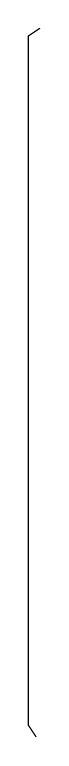
\begin{tikzpicture}[x=1cm,y=1cm]\draw (0.15,9)--(0,8.9)--(0,0.15)--(0.1,0);\end{tikzpicture}}}
\uline{Corollaire 2.5} : Il existe une suite spectrale fonctorielle en $F$ et en $X$ (objet de $C$) :
\[
H^{p+q}(C^{\sim}/X,F)\Longleftarrow\check H^p(X,\mathcal H^q(F))
\]
Cette suite spectrale fournit, lorsque $X$ varie dans $C$, la suite spectrale de préfaisceaux :
\[
\mathcal H^{p+q}(F)\Longleftarrow\check{\mathcal H}^{p}(\mathcal H^q(F))
\]
Ces suites spectrales fournissent des morphismes fonctoriels :
\margin{$\unsure{\checkmark}$}
\[
\Phi^q(F):\check{\mathcal H}^{q}(\mathcal H^0(F))\longrightarrow\mathcal H^q(F)
\]
\[
\Phi_X^q(F):\check H^q(\unsure{E|S}\ X,\mathcal H^0(F))\longrightarrow H^q(X,F)
\]
Les morphismes $\Phi^q$ et $\Phi_X^q$ sont des isomorphismes lorsque $q$ égale $0$ ou $1$. Les morphismes $\Phi^2$ et $\Phi_X^2$ sont des monomorphismes.

Plus généralement, lorsque les préfaisceaux $\mathcal H^i(F)$ sont nuls pour $0<i<n$, les morphismes $\Phi^q(F)$ et $\Phi_X^q(F)$ sont des isomorphismes pour $0\leq q\leq n$ et des monomorphismes pour $q=n+1$.

\uline{Preuve} : La première suite spectrale s'obtient en passant à la limite inductive dans la suite spectrale de la proposition 2.3 sur les
\[\ldots/\ldots\]
